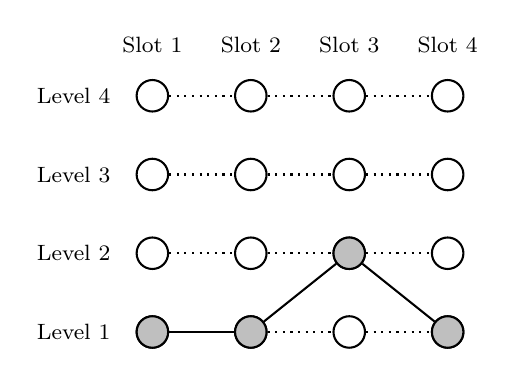
\begin{tikzpicture}
  [
  font=\footnotesize, line width=0.75pt, draw=black,
  subblock/.style={circle, inner sep = 0pt, minimum size = 4mm, draw=black}
  ]

\foreach \x in {1,2,3,4} {
  \foreach \y in {1,2,3,4} {
    \node[subblock] (x{\x}y{\y}) at (1.25*\x - 1.25,\y) {};
  }
  \node (s{\x}) at (1.25*\x - 1.25,4.65) {Slot~\x};
}
\foreach \y in {1,2,3,4} {
  \node (l{\y}) at (-1,\y) {Level~\y};
}

\foreach \y in {1,2,3,4} {
  \draw[dotted](x{1}y{\y}) -- (x{2}y{\y});
  \draw[dotted](x{2}y{\y}) -- (x{3}y{\y});
  \draw[dotted](x{3}y{\y}) -- (x{4}y{\y});
}

\node[subblock,fill=lightgray] (px1y1) at (0,1) {};
\node[subblock,fill=lightgray] (px2y1) at (1.25,1) {}
  edge (px1y1);
\node[subblock,fill=lightgray] (px3y2) at (2.5,2) {}
  edge (px2y1);
\node[subblock,fill=lightgray] (px4y1) at (3.75,1) {}
  edge (px3y2);

\end{tikzpicture}
